% Concept and Design
%
\chapter{Concept and Design}\label{ch:concept_and_design}

This chapter presents the concept and design of the investigative work of this thesis. The previous chapter outlined research direction, requirements, and objectives of the system to be developed. Based on these requirements, this chapter discusses the design of the system preceeding implementation in Chapter~\ref{ch:implementation}. 

The main purpose of the design is to develop a suitable \gls{ac:ssr-x} pulse compression radar simulation and accompanying evaluation framework to facilitate the investigation of power amplifier nonlinearity effects and predistortion to counteract these. As elaborated in the objectives analysis section~\ref{sec:objectives_analysis}, this involves first developing a generic pulse compression radar simulation -- modelling the main components of the real \gls{ac:ssr-x} pulse compression radar system, as well as nonlinear power amplifier and predistorter models. Then, the simulation is tailored to accurately emulate the real system using measurements performed on the physical hardware. The simulation serves as a boilerplate framework to apply and test predistortion algorithms preceeding any implementation on the real system. As such, evaluation criteria are necessary for judgement of the performance of predistortion. This involves numerical comparison predicated on the different \glspl{ac:kpi} mentioned in Chapter~\ref{ch:requirements_analysis}. 

The design of the components of the system are of a modular structure in accordance with NFR2 in in section~\ref{sec:reqs_overview}. This ensures an easily maintable and extendable system. Each component of the pulse compression chain, the power amplifier, and predistorter model are developed independently from each other as modules within the simulation. They interact together, but can be modified and finetuned separately. As such, observed performance differences between different power amplifier and predistorter models for comparison can be strictly attributed to changes in those modules, not to other simulation conditions. This enables a reliable framework for evaluation.

\section{Overall Approach}

The overall approach of this thesis is to design and implement the \gls{ac:ssr-x} pulse compression radar simulation and use it as a test environment for evaluating and understanding the effects of power amplifier nonlinearity and predistortion preceeding hardware implementation. Development of the simulation is the core of the work, enabling a test sandbox to easily configure and experiment with nonlinearity effects and predistortion results. Through refinement by measurements on the hardware, the true behaviour of the system can be closely modelled. Once the best predistortion technique is found in simulation, the experiment can be conducted on the hardware to observe for real world performance gains. 

The general workflow of this thesis is shown in the following steps:

\begin{enumerate}
  \item Design and implement a generic \gls{ac:ssr-x} pulse compression radar simulation -- including main components of the pulse compression system, the power amplifier, and predistorter
  \item Perform measurements on the \gls{ac:ssr-x} pulse compression radar hardware to better understand the behaviour of the real system
  \item Finetune the simulation using measurement observations and findings for accurate representation of the system
  \item Apply evaluation criteria to determine the performance improvement by predistortion in simulation
  \item Apply the simulated predistorter on the \gls{ac:ssr-x} pulse compression radar hardware to confirm real performance improvement
\end{enumerate}

The simulation and its accompanying evaluative aspects are implemented as a python script, in accordance with NFR1 in section~\ref{sec:reqs_overview}. This is conducive to rapid development and implementation ease due to the abundance of useful provided libraries. Real system hardware measurements however will be performed in a lab environment using measurement equipment, such as oscilloscopes and spectrum analysers.   

The application of evaluation criteria for predistorter performance is based on numerically comparing \gls{ac:kpi} metrics listed in section~\ref{sec:reqs_overview}. In the simulation, this evaluation will dictate how much predistortion theoretically enhances performance by cancelling adverse nonlinearities. When the predistorter is then implemented on the physcial hardware, the evaluation can again be performed using measured \glspl{ac:kpi} -- verifying performance improvement in practicality.

\section{System Architecture}\label{sec:system_architecture}

The system architecture is designed as a modular \gls{ac:ssr-x} pulse compression radar simulation system and evaluation framework. The primary components entail the pulse compression radar system, nonlinear power amplifier, predistorter, and evaluative result logs and plots. Each of these primary components, including their relationship with one another, is elaborated on in the following subsections.

\begin{figure}[tb]
  \centering
  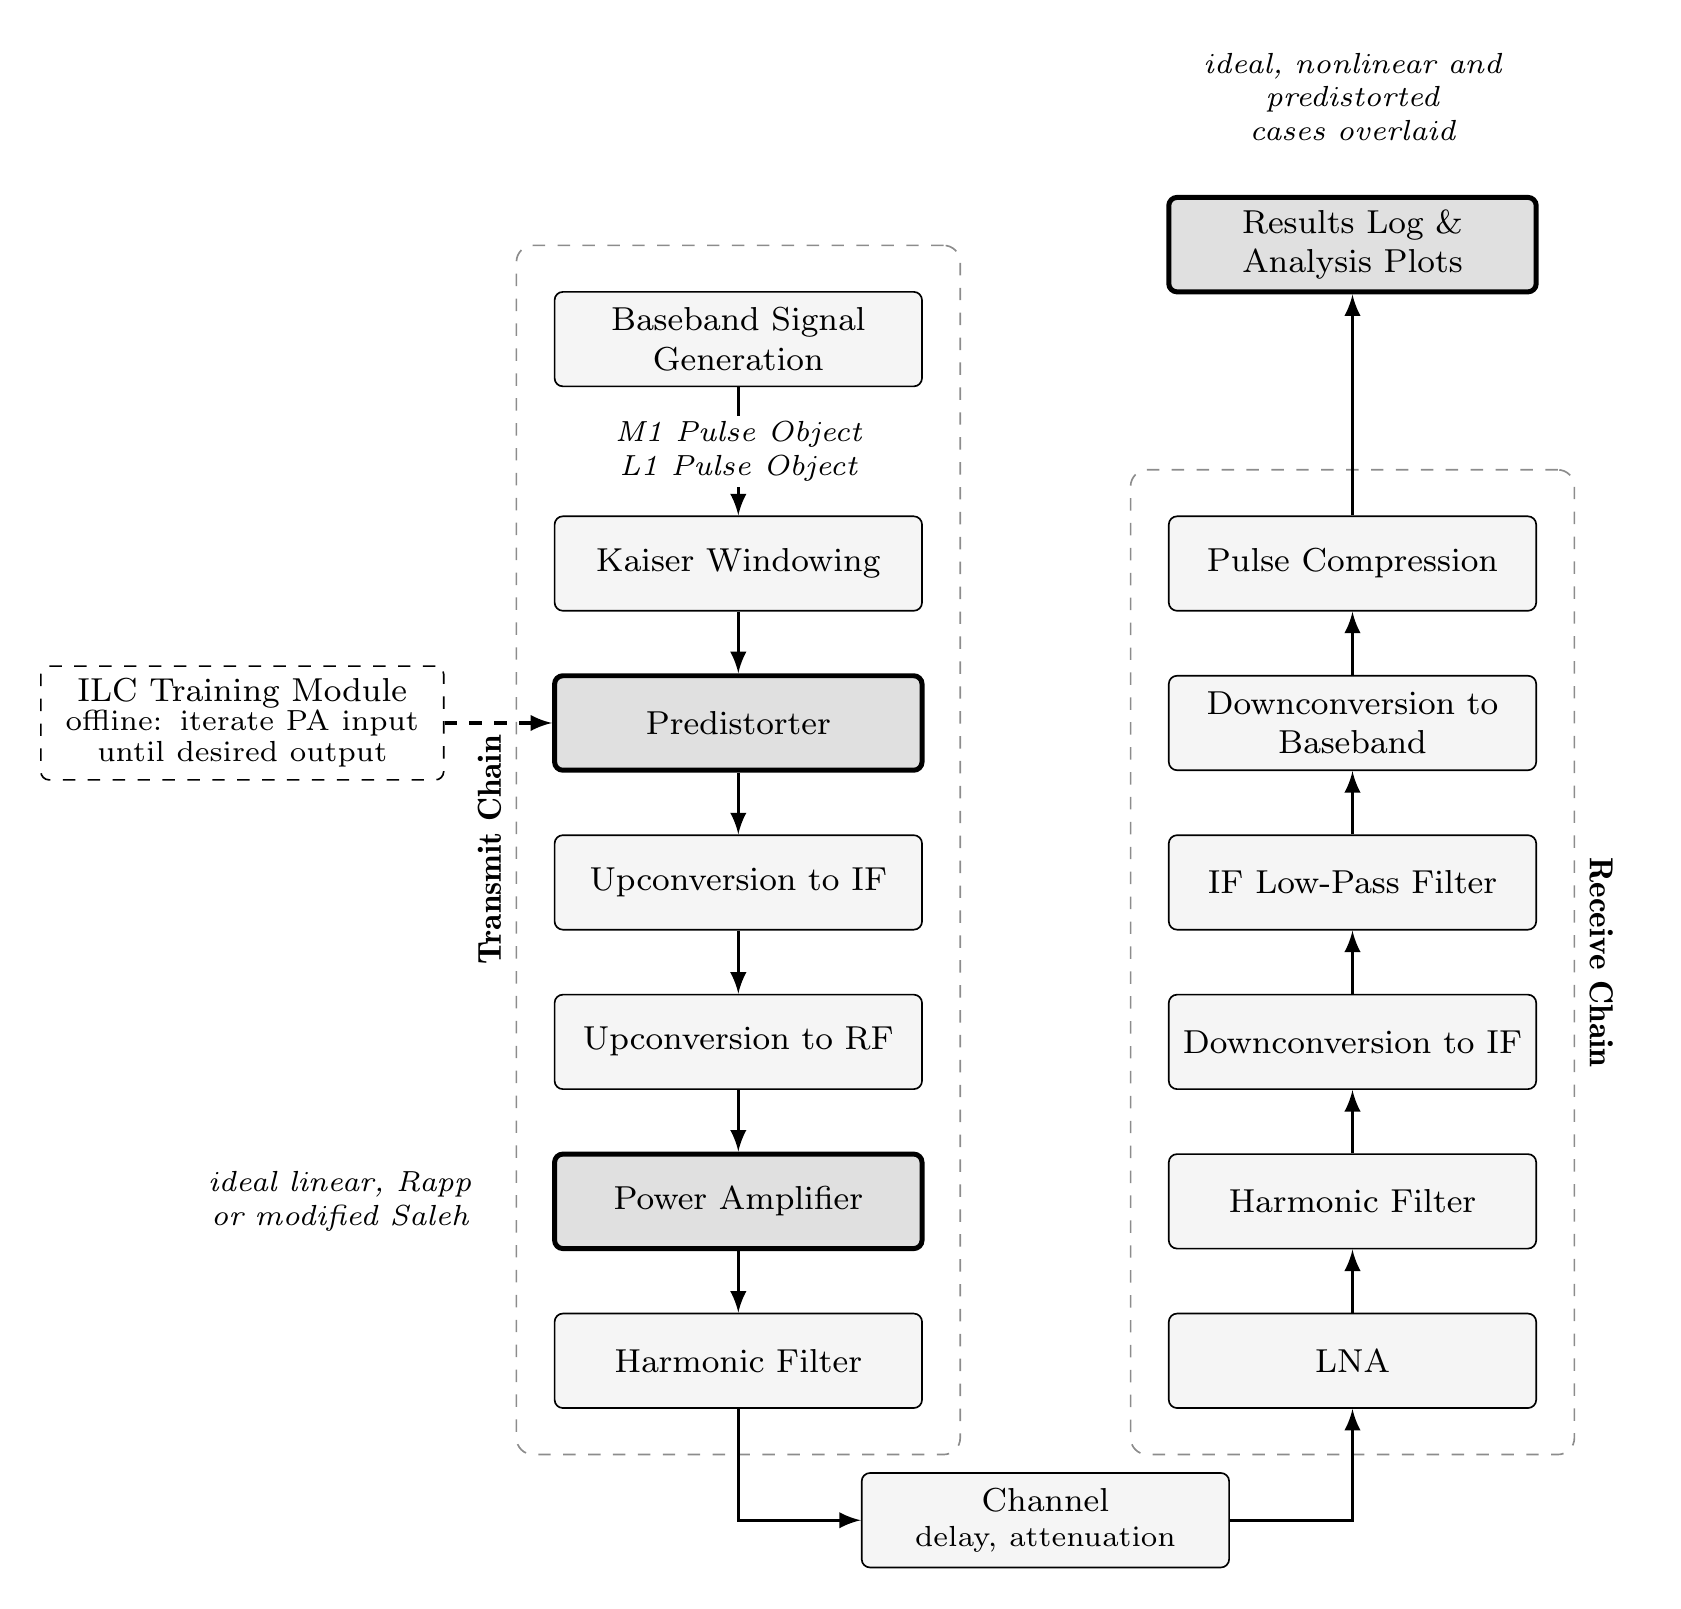
\includegraphics[width=0.9\textwidth]{Figures/ConceptAndDesign/Programme_flow}
  \caption{Programme flow of pulse compression radar simulation}
  \label{fig:programme_flow}
\end{figure}

\subsection{Pulse Compression Radar Chain Design}

The pulse compression radar system serves as the backbone of the entire simulation. It comprises each of the main building blocks of the pulse compression system, namely the transmit chain, channel, and receive chain. Each of these building blocks consists of further subcomponents. In the transmit chain, the submodules are baseband signal generation and Kaiser windowing, predistortion (explained in section~\ref{sec:predistorter_design}), upconversion to \gls{ac:if} and \gls{ac:rf} respectively, amplification (initially via an ideal linear amplifier, though extended in section~\ref{sec:power_amp_design}), and harmonic filter before transmission. In the receive chain, the submodules are the \gls{ac:lna}, harmonic filter, downconversion to \gls{ac:if}, \gls{ac:if} low pass filter, downconversion to baseband, and finally pulse compression. The modules have been listed in chronological order where the output of one module becomes the input of the next. 

Traversing each of these submodules are the radar pulse signals themselves. \gls{ac:ssr-x} pulse compression radar signals of interest for the thesis' investigation are the \gls{ac:lfm} medium (M1) and long (L1) pulses, where the M1 pulse has a $\SI{4}{\micro\second}$ duration and $\SI{10}{\mega\hertz}$ bandwidth and the L1 pulse a $\SI{25}{\micro\second}$ duration and $\SI{5}{\mega\hertz}$ bandwidth. 

The pulses are first generated in the baseband signal generation module and must be passed and processed through the entire signal chain until the pulse compression submodule. The submodules are thus designed as modular Python functions, and the pulses are sequentially processed as Python objects by each function -- in accordance with FR2 in section~\ref{sec:reqs_overview}. A complete programme flow diagram of the design is seen in Figure~\ref{fig:programme_flow}.

\subsection{Power Amplifier Module Design}\label{sec:power_amp_design}

The power amplifier module models the nonlinearity effects of the power amplifier chain of the system. It essentially stands as the (nonlinear) amplification module in the transmit chain of the pulse compression radar simulation -- in essence, the module is designed as Python function and is depicted in Figure~\ref{fig:programme_flow}. Section~\ref{sec:pa_models} elucidates various proven power amplifier mathematical models from theory. The function applies the mathematical model on the input pulse signal to obtain the distorted output pulse afflicted with nonlinearity effects. 

Due to its simplicity and reliability when extrapolating towards saturation, the Rapp model -- along with Honkanen and H\"aggman's \gls{ac:am-pm} extension -- is chosen as the main mathematical model. Details of the Rapp model are found in section~\ref{sec:rapp_model}. As a secondary model, the modified Saleh model -- introduced by O'Droma, Meza and Lei and seen in section~\ref{sec:rapp_model} -- is chosen due to it being the best performing model when extending into saturation. The two models can be compared against measurements performed on the real hardware to find the most suitable option. The usage of these two models satisfies FR3 in section~\ref{sec:reqs_overview}.

\subsection{Predistorter Module Design}\label{sec:predistorter_design}

Analogous to the power amplifier module, the predistorter module is a Python function serving as a submodule in the transmit chain -- seen in Figure~\ref{fig:programme_flow}. It is inserted directly after baseband signal generation and windowing. Section~\ref{sec:predistortion} introduces three types of predistortion -- baseband, \gls{ac:if}, and \gls{ac:rf} predistortion. The predistorter module design will focus on digital baseband predistortion due to its simplicity, reconfigurability, and ease of implementing adaptivity. Three baseband predistortion approaches are discussed in section~\ref{sec:baseband_predistortion} -- \gls{ac:ila}, \gls{ac:dla}, and \gls{ac:ilc}. Of the three, \gls{ac:ilc} is the most suitable approach for pulse compression radar. As the radar pulses remain the same for every transmission -- the M1 and L1 pulses respectively -- the optimal predistorter result can be computed once and saved. No model of the power amplifier itself nor its inverse characteristic are required like the \gls{ac:ila} and \gls{ac:dla} approaches. However, the design is only made adaptive by periodically recomputing the optimal predistorter result via \gls{ac:ilc}. This only concerns implementation of the predistorter module on real hardware, as the simulation is unaffected by the factors that adaptivity aims to counter i.~e. aging and temperature effects.

Hence, \gls{ac:ilc} is chosen for the predistorter module design, fulfilling FR4 in section~\ref{sec:reqs_overview}. The predistorter module function outputs the precalculated optimal predistorted pulse depending on its input, either the M1 or L1 pulse. The optimal predistorter result is computed by running a training module preceeding full programme flow through the pulse compression radar simulation. The training module iteratively runs the \gls{ac:ilc} algorithm by passing the input pulse through the power amplifier module and adjusting it until the desired output is achieved. Once the desired output is obtained, it is saved as the predistorter output and loaded when the predistorter module is called during a full programme run.   

\subsection{Results Logs and Plots}\label{sec:results_logs_and_plots}

The plotting and results logs are critical components for the determination of nonlinearity effects and performance gain from predistortion. The requirements in section~\ref{sec:reqs_overview} define the required plots and recording of \glspl{ac:kpi} for this purpose. FR5 states that analysis plots are required for three cases -- ideal, nonlinear, and predistorted -- overlayed on each other for direct visual comparison. FR6, FR7, FR8, and FR9 define the plots to be generated, including quantitative values of \glspl{ac:kpi} the plots should display. The generated plots, including their \glspl{ac:kpi}, entail the following:

\begin{enumerate}
  \item Spectrum plots at each stage of the simulation with \glspl{ac:kpi} of main lobe peak amplitude, \gls{ac:psl}, \gls{ac:isl}, and second harmonic main lobe level
  \item Pulse compression plot of with \glspl{ac:kpi} of main lobe peak amplitude, \gls{ac:psl}, and \gls{ac:isl}
  \item Power amplifier \gls{ac:am-am} plots with \gls{ac:kpi} of \qty{1}{\decibel} compression point
  \item Power amplifier \gls{ac:am-pm} plots with \gls{ac:kpi} of total phase deviation
\end{enumerate}

As stated, the above analysis plots will overlay the ideal, nonlinear, and predistorted curves -- including markers for their defined \glspl{ac:kpi}. The results logs will print the \gls{ac:kpi} numerical values and their differences for the three cases in a log file for evaluation. The results log and plot generation are respectively designed as python functions. These functions are called at the end of the simulation, following execution of all stages of the pulse compression radar simulation. They are seen as the final stage depicted in Figure~\ref{fig:programme_flow}.

\section{Evaluation Criteria}

Evaluation here is two-fold. Firstly, evaluation refers to determining the extent of detrimental nonlinearity and performance gain via predistortion. Secondarily, evaluation also refers to determining whether the developed simulation and thesis work are satisfactory -- in fulfillment with the requirements defined in section~\ref{sec:reqs_overview}. This requirements fulfillment evaluation is performed in Chapter~\ref{ch:evaluation}. 

Regarding the nonlinearity extent and performance gain, evaluation is predicated on the generated results logs and plots elaborated in section~\ref{sec:results_logs_and_plots}. The evaluation is purely investigative and numerically grounded. The extent of power amplifier nonlinearity will be quantitatively determined by comparing differences in \gls{ac:kpi} values between the ideal (linear) and nonlinear case. On the other hand, the extent of predistortion performance gain is quantitively deduced by comparing differences in between nonlinear and predistorted cases -- to examine the extent of nonlinearity reversal -- and between linear and predistorted cases -- to examine how close predistortion can reach the ideal linearity. The evaluation will be performed in Chapter~\ref{ch:evaluation} in tabular form to clearly see numerical discrepancies between the three cases. The descriptive evaluation obtained from these results will follow. 


